% Font options: 10pm, 11pt, 12pt
% Align headings left instead of center: nocenter
\documentclass[xcolor=x11names,compress]{beamer}\usepackage[]{graphicx}\usepackage[]{color}
%% maxwidth is the original width if it is less than linewidth
%% otherwise use linewidth (to make sure the graphics do not exceed the margin)
\makeatletter
\def\maxwidth{ %
  \ifdim\Gin@nat@width>\linewidth
    \linewidth
  \else
    \Gin@nat@width
  \fi
}
\makeatother

\definecolor{fgcolor}{rgb}{0.345, 0.345, 0.345}
\newcommand{\hlnum}[1]{\textcolor[rgb]{0.686,0.059,0.569}{#1}}%
\newcommand{\hlstr}[1]{\textcolor[rgb]{0.192,0.494,0.8}{#1}}%
\newcommand{\hlcom}[1]{\textcolor[rgb]{0.678,0.584,0.686}{\textit{#1}}}%
\newcommand{\hlopt}[1]{\textcolor[rgb]{0,0,0}{#1}}%
\newcommand{\hlstd}[1]{\textcolor[rgb]{0.345,0.345,0.345}{#1}}%
\newcommand{\hlkwa}[1]{\textcolor[rgb]{0.161,0.373,0.58}{\textbf{#1}}}%
\newcommand{\hlkwb}[1]{\textcolor[rgb]{0.69,0.353,0.396}{#1}}%
\newcommand{\hlkwc}[1]{\textcolor[rgb]{0.333,0.667,0.333}{#1}}%
\newcommand{\hlkwd}[1]{\textcolor[rgb]{0.737,0.353,0.396}{\textbf{#1}}}%
\let\hlipl\hlkwb

\usepackage{framed}
\makeatletter
\newenvironment{kframe}{%
 \def\at@end@of@kframe{}%
 \ifinner\ifhmode%
  \def\at@end@of@kframe{\end{minipage}}%
  \begin{minipage}{\columnwidth}%
 \fi\fi%
 \def\FrameCommand##1{\hskip\@totalleftmargin \hskip-\fboxsep
 \colorbox{shadecolor}{##1}\hskip-\fboxsep
     % There is no \\@totalrightmargin, so:
     \hskip-\linewidth \hskip-\@totalleftmargin \hskip\columnwidth}%
 \MakeFramed {\advance\hsize-\width
   \@totalleftmargin\z@ \linewidth\hsize
   \@setminipage}}%
 {\par\unskip\endMakeFramed%
 \at@end@of@kframe}
\makeatother

\definecolor{shadecolor}{rgb}{.97, .97, .97}
\definecolor{messagecolor}{rgb}{0, 0, 0}
\definecolor{warningcolor}{rgb}{1, 0, 1}
\definecolor{errorcolor}{rgb}{1, 0, 0}
\newenvironment{knitrout}{}{} % an empty environment to be redefined in TeX

\usepackage{alltt}
%\documentclass[xcolor=x11names,compress,handout]{beamer}
\usepackage[]{graphicx}
\usepackage[]{color}
\usepackage{booktabs}
\usepackage{hyperref}
\usepackage{tikz}
\usepackage{multirow}
\usepackage{multicol}
\usepackage{dcolumn}
\usepackage{bigstrut}
\usepackage{amsmath} 
\usepackage{xcolor,colortbl}
\usepackage{amssymb}
%\newcommand{\done}{\cellcolor{teal}#1}

%% Beamer Layout %%%%%%%%%%%%%%%%%%%%%%%%%%%%%%%%%%
\useoutertheme[subsection=false,shadow]{miniframes}
\useinnertheme{default}
\usefonttheme{serif}
\usepackage{Arev}
\usepackage{pdfpages}

\setbeamerfont{title like}{shape=\scshape}
\setbeamerfont{frametitle}{shape=\scshape, size=\normalsize}

\definecolor{dkblue}{RGB}{0,0,102}

\setbeamercolor*{lower separation line head}{bg=dkblue} 
\setbeamercolor*{normal text}{fg=black,bg=white} 
\setbeamercolor*{alerted text}{fg=red} 
\setbeamercolor*{example text}{fg=black} 
\setbeamercolor*{structure}{fg=black} 
 
\setbeamercolor*{palette tertiary}{fg=black,bg=black!10} 
\setbeamercolor*{palette quaternary}{fg=black,bg=black!10} 

\renewcommand{\(}{\begin{columns}}
\renewcommand{\)}{\end{columns}}
\newcommand{\<}[1]{\begin{column}{#1}}
\renewcommand{\>}{\end{column}}

\setbeamertemplate{navigation symbols}{} 
\setbeamertemplate{footline}[frame number]
\setbeamertemplate{caption}{\raggedright\insertcaption\par}

\setbeamersize{text margin left=5pt,text margin right=5pt}

%%%%%%%%%%%%%%%%%%%%%%%%%%%%%%%%%%%%%%%%%%%%%%%%%%




\title{FLS 6441 - Methods III: Explanation and Causation}
\subtitle{Week 1 - Review}
\author{Jonathan Phillips}
\date{February 2019}
\IfFileExists{upquote.sty}{\usepackage{upquote}}{}
\begin{document}

\frame{\titlepage}

\section{Introduction}

\begin{frame}
\frametitle{Course Objectives}
\begin{enumerate}
\item temp
\end{enumerate}
\end{frame}

\section{Probability}

\begin{frame}
\frametitle{Data}
\begin{enumerate}
\item We work with variables, which VARY!
\end{enumerate}
\begin{multicols}{2}
% latex table generated in R 3.5.2 by xtable 1.8-3 package
% Sat Mar 02 09:47:06 2019
\begin{table}[ht]
\centering
\begin{tabular}{rr}
  \hline
 & Variable \\ 
  \hline
1 & 1.68 \\ 
  2 & 0.25 \\ 
  3 & 1.30 \\ 
  4 & -1.12 \\ 
  5 & -0.80 \\ 
  6 & -0.54 \\ 
  7 & -0.92 \\ 
  8 & 0.53 \\ 
  9 & 1.11 \\ 
  10 & -0.63 \\ 
   \hline
\end{tabular}
\end{table}

\columnbreak
\begin{knitrout}
\definecolor{shadecolor}{rgb}{0.969, 0.969, 0.969}\color{fgcolor}
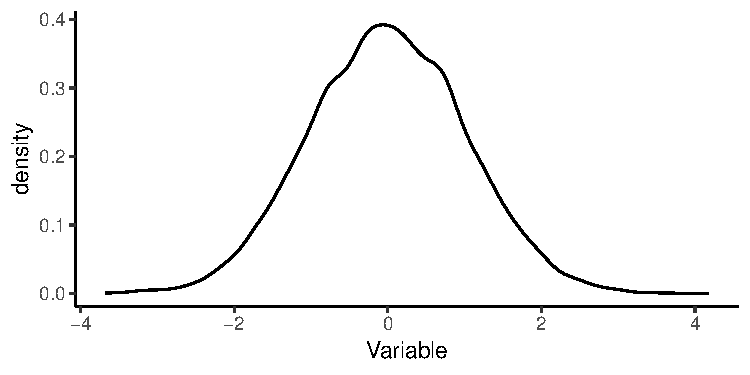
\includegraphics[width=\maxwidth]{figure/var2-1} 

\end{knitrout}
\end{multicols}
\end{frame}

% Bayes Rule: P(AnB)=P(A|B)*P(B)
% Independence: P(AnB)=P(A)*P(B) -> AIndepB. P(A|B)=P(A)
% E(x)=for random variable; (weighted) average is for sample. Same in large N/many repeated. Lecture 2, slide 69

\section{What does Regression do?}

\begin{frame}
\frametitle{Regression}
\begin{itemize}
\item Regression identifies the line through the data that minimizes the sum of squared vertical distances 
\pause
\item $y_i = \alpha + \beta X_i + \epsilon_i$
\pause
\end{itemize}
\begin{multicols}{2}
%Insert graph with vertical lines
\begin{knitrout}
\definecolor{shadecolor}{rgb}{0.969, 0.969, 0.969}\color{fgcolor}
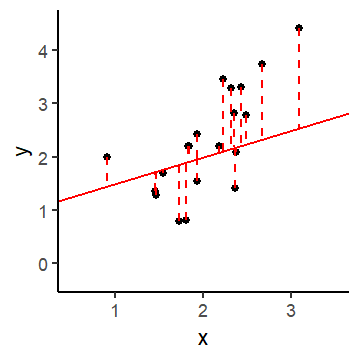
\includegraphics[width=\maxwidth]{figure/graph_reg1-1} 

\end{knitrout}
\columnbreak
\end{multicols}
\end{frame}


\begin{frame}
\frametitle{Regression}
\begin{itemize}
\item Regression identifies the line through the data that minimizes the sum of squared vertical distances 
\item $y_i = \alpha + \beta X_i + \epsilon_i$
\end{itemize}
\begin{multicols}{2}
%Insert graph with vertical lines
\begin{knitrout}
\definecolor{shadecolor}{rgb}{0.969, 0.969, 0.969}\color{fgcolor}

\includegraphics[width=\maxwidth]{figure/graph_reg2-1} 

\end{knitrout}
\columnbreak
\end{multicols}
\end{frame}


\begin{frame}
\frametitle{Regression}
\begin{itemize}
\item Regression identifies the line through the data that minimizes the sum of squared vertical distances 
\item $y_i = \alpha + \beta X_i + \epsilon_i$
\end{itemize}
\begin{multicols}{2}
%Insert graph with vertical lines
\begin{knitrout}
\definecolor{shadecolor}{rgb}{0.969, 0.969, 0.969}\color{fgcolor}

\includegraphics[width=\maxwidth]{figure/graph_reg3-1} 

\end{knitrout}
\columnbreak
\begin{itemize}
\item Sum of Squared distances = 10.39
\end{itemize}
\end{multicols}
\end{frame}

\begin{frame}
\frametitle{Regression}
\begin{itemize}
\item Regression identifies the line through the data that minimizes the sum of squared vertical distances 
\item $y_i = \alpha + \beta X_i + \epsilon_i$
\end{itemize}
\begin{multicols}{2}
%Insert graph with vertical lines
\begin{knitrout}
\definecolor{shadecolor}{rgb}{0.969, 0.969, 0.969}\color{fgcolor}

\includegraphics[width=\maxwidth]{figure/graph_reg4-1} 

\end{knitrout}
\columnbreak
\end{multicols}
\end{frame}

\begin{frame}
\frametitle{Regression}
\begin{itemize}
\item Regression identifies the line through the data that minimizes the sum of squared vertical distances 
\item $y_i = \alpha + \beta X_i + \epsilon_i$
\end{itemize}
\begin{multicols}{2}
%Insert graph with vertical lines
\begin{knitrout}
\definecolor{shadecolor}{rgb}{0.969, 0.969, 0.969}\color{fgcolor}

\includegraphics[width=\maxwidth]{figure/graph_reg5-1} 

\end{knitrout}
\columnbreak
\begin{itemize}
\item Sum of Squared distances = 9.19
\end{itemize}
\end{multicols}
\end{frame}


%epsilon larger when more dispersed around line with same slope

\begin{frame}
\frametitle{Regression}
\begin{itemize}
\item Regression is a \textbf{Conditional Expectation Function}
\pause
\item Conditional on $x$, what is our expectation (mean value) of $y$?
\pause
\item $E(y|x)$
\pause
\item When age is 20 ($x=40$), the average salary is R1.000 ($y=1.000$)
\item When age is 40 ($x=40$), the average salary is R2.000 ($y=2.000$)
\end{itemize}
\end{frame}

\begin{frame}
\frametitle{Regression}
\begin{itemize}
\item Regression is a \textbf{Conditional Expectation Function}: $E(y|x)$
\pause
\item It predicts the \textbf{mean}, not the median, not the minimum, not the maximum
\end{itemize}
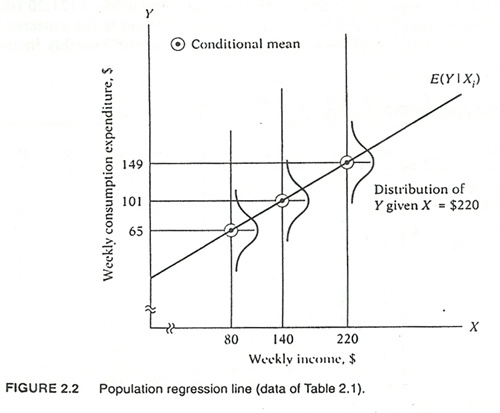
\includegraphics[width=0.75\textwidth]{CEF.jpg}
\end{frame}

\begin{frame}
\frametitle{Regression}
$$\hat{\beta_1}=\frac{\sum_i (x_i - \bar{x})(y_i - \bar{y})}{\sum_i (x_i - \bar{x})^2}$$
$$\hat{\beta_0}=\bar{y} - \hat{\beta_1} \bar{x}$$
\end{frame}



\begin{frame}
\frametitle{Regression}
\begin{itemize}
\item Regression with two variables is very similar to calculating correlation
\pause
\item $\hat{\beta}=cor(x,y) * \frac{\sigma_Y}{\sigma_X}$
\pause
\item It's \textit{identical} if we standardize both variables first ($\frac{(x-\bar{x})}{\sigma_x}$)
\pause
\end{itemize}
\begin{multicols}{2}
\begin{knitrout}
\definecolor{shadecolor}{rgb}{0.969, 0.969, 0.969}\color{fgcolor}
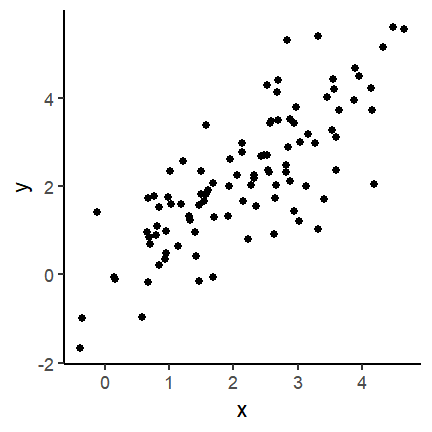
\includegraphics[width=\maxwidth]{figure/corr_regn_fig1-1} 

\end{knitrout}
\columnbreak
\end{multicols}
\end{frame}

\begin{frame}
\frametitle{Regression}
\begin{itemize}
\item Regression with two variables is very similar to calculating correlation:
\item $\hat{\beta}=cor(x,y) * \frac{\sigma_Y}{\sigma_X}$
\item It's \textit{identical} if we standardize both variables first ($\frac{(x-\bar{x})}{\sigma_x}$)
\end{itemize}
\begin{multicols}{2}
\begin{knitrout}
\definecolor{shadecolor}{rgb}{0.969, 0.969, 0.969}\color{fgcolor}
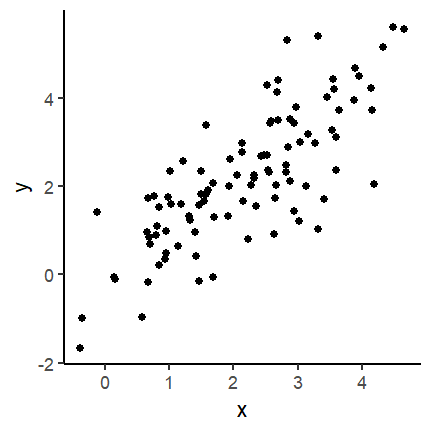
\includegraphics[width=\maxwidth]{figure/corr_regn_fig2-1} 

\end{knitrout}
\columnbreak
\begin{itemize}
\item Correlation is 0.781
\pause
\item Regression Results:
\end{itemize}
% latex table generated in R 3.5.2 by xtable 1.8-3 package
% Sat Mar 02 09:47:18 2019
\begin{table}[ht]
\centering
\begin{tabular}{rlr}
  \hline
 & term & estimate \\ 
  \hline
1 & (Intercept) & 0.006 \\ 
  2 & x & 1.008 \\ 
   \hline
\end{tabular}
\end{table}

\end{multicols}
\end{frame}

\begin{frame}
\frametitle{Regression}
\begin{itemize}
\item Regression with two variables is very similar to calculating correlation:
\item $\hat{\beta}=cor(x,y) * \frac{\sigma_Y}{\sigma_X}$
\item It's \textit{identical} if we standardize both variables first ($\frac{(x-\bar{x})}{\sigma_x}$)
\end{itemize}
\begin{multicols}{2}
\begin{knitrout}
\definecolor{shadecolor}{rgb}{0.969, 0.969, 0.969}\color{fgcolor}
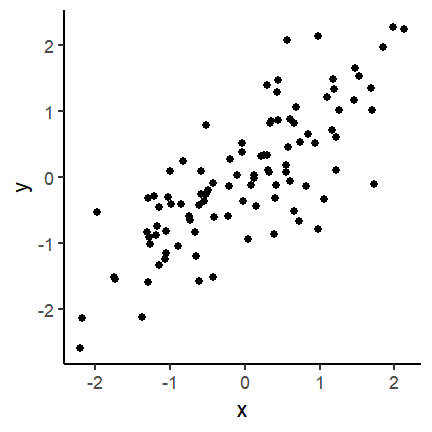
\includegraphics[width=\maxwidth]{figure/corr_regn_fig3-1} 

\end{knitrout}
\columnbreak
\begin{itemize}
\item Correlation is 0.781
\item Standardized Regression Results:
\end{itemize}
% latex table generated in R 3.5.2 by xtable 1.8-3 package
% Sat Mar 02 09:47:19 2019
\begin{table}[ht]
\centering
\begin{tabular}{rlr}
  \hline
 & term & estimate \\ 
  \hline
1 & (Intercept) & 0.000 \\ 
  2 & x & 0.781 \\ 
   \hline
\end{tabular}
\end{table}

\end{multicols}
\end{frame}

\begin{frame}
\frametitle{Regression}
\begin{itemize}
\item Regression with \textbf{multiple} variables is very similar to calculating \textbf{partial} correlation:
\pause
\item Just a small difference in the denominator (how we standardize the measure)
\pause
\end{itemize}
$$\beta_{x_1} = \frac{r_{yx_1} - r_{yx_2}r_{x_1x_2}}{1-r^2_{x_1x_2}}$$
$$r_{yx_1|x_2} = \frac{r_{yx_1} - r_{yx_2}r_{x_1x_2}}{\sqrt{(1-r^2_{yx_2})(1-r^2_{x_1x_2})}}$$
\begin{itemize}
\item \textbf{There is no magic in regression, it's just correlation}
\end{itemize}
\end{frame}

\begin{frame}
\frametitle{Regression}
\begin{itemize}
\item We \textbf{NEVER} know the true value of $\beta$
\pause
\item We \textbf{estimate a distribution} for $\beta$
\end{itemize}
\begin{knitrout}
\definecolor{shadecolor}{rgb}{0.969, 0.969, 0.969}\color{fgcolor}
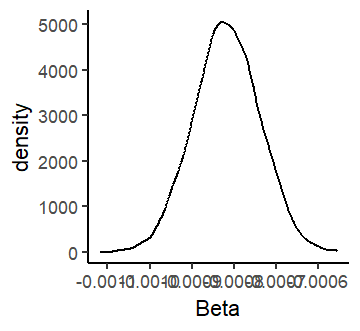
\includegraphics[width=\maxwidth]{figure/beta_dist-1} 

\end{knitrout}
\end{frame}

\begin{frame}
\frametitle{Regression}
\begin{itemize}
\item We \textbf{NEVER} know the true value of $\beta$
\item We \textbf{estimate a distribution} for $\beta$
\end{itemize}
\begin{knitrout}
\definecolor{shadecolor}{rgb}{0.969, 0.969, 0.969}\color{fgcolor}
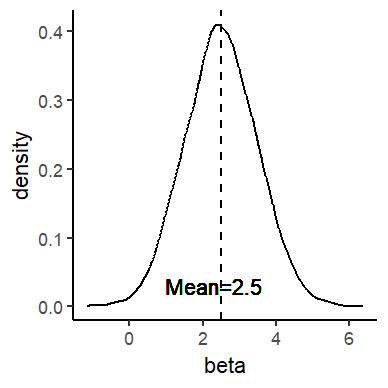
\includegraphics[width=\maxwidth]{figure/beta_dist2-1} 

\end{knitrout}
\end{frame}

\begin{frame}
\frametitle{Regression}
\begin{itemize}
\item We \textbf{NEVER} know the true value of $\beta$
\item We \textbf{estimate a distribution} for $\beta$
\end{itemize}
\begin{knitrout}
\definecolor{shadecolor}{rgb}{0.969, 0.969, 0.969}\color{fgcolor}
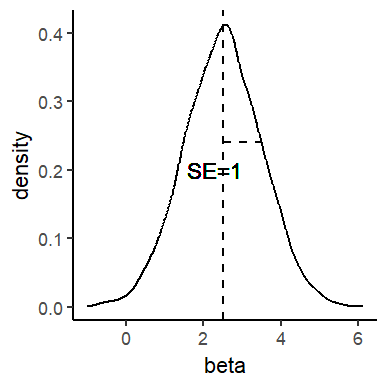
\includegraphics[width=\maxwidth]{figure/beta_dist3-1} 

\end{knitrout}
\end{frame}

\begin{frame}
\frametitle{Regression}
\begin{itemize}
\item We \textbf{NEVER} know the true value of $\beta$
\item We \textbf{estimate a distribution} for $\beta$
\end{itemize}
\begin{knitrout}
\definecolor{shadecolor}{rgb}{0.969, 0.969, 0.969}\color{fgcolor}
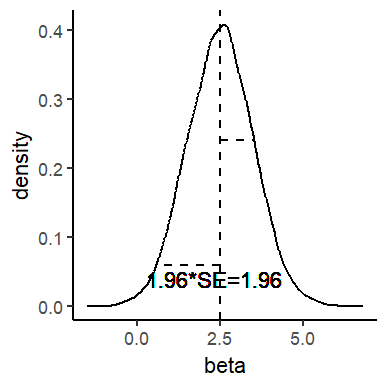
\includegraphics[width=\maxwidth]{figure/beta_dist4-1} 

\end{knitrout}
\end{frame}

\begin{frame}
\frametitle{Regression}
\begin{itemize}
\item We \textbf{NEVER} know the true value of $\beta$
\item We \textbf{estimate a distribution} for $\beta$
\end{itemize}
\begin{knitrout}
\definecolor{shadecolor}{rgb}{0.969, 0.969, 0.969}\color{fgcolor}
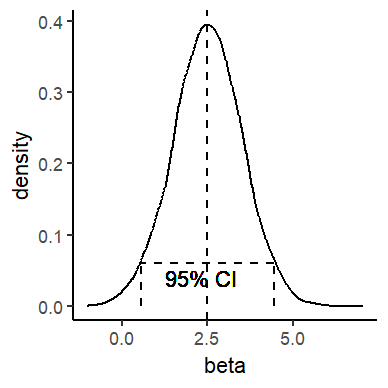
\includegraphics[width=\maxwidth]{figure/beta_dist5-1} 

\end{knitrout}
\end{frame}


\section{Guide to Designing Regressions}

\begin{frame}
\frametitle{Regression Guide}
\begin{enumerate}
\item \textbf{Choose variables and measures:} To test a specific hypothesis
\item \textbf{Choose a Model/Link Function:} Should match the data type of your outcome variable
\item \textbf{Choose Covariates:} To match your strategy of inference
\item \textbf{Choose Fixed Effects:} To focus on a specific level of variation
\item \textbf{Choose Error Structure:} To match known dependencies/clustering in the data
\item \textbf{Interpret the coefficients:} Depending on the type/scale of the explanatory variable
\end{enumerate}
\end{frame}

\begin{frame}
\frametitle{2. Regression Models}
The Regression Model reflects the data type of the outcome variable:
\begin{itemize}
\item Continuous -> Ordinary Least Squares  
\begin{knitrout}
\definecolor{shadecolor}{rgb}{0.969, 0.969, 0.969}\color{fgcolor}\begin{kframe}
\begin{alltt}
\hlkwd{zelig}\hlstd{(Y} \hlopt{~} \hlstd{X,}\hlkwc{data}\hlstd{=d,}\hlkwc{model}\hlstd{=}\hlstr{"ls"}\hlstd{)}
\end{alltt}
\end{kframe}
\end{knitrout}
\item Binary -> Logit  
\begin{knitrout}
\definecolor{shadecolor}{rgb}{0.969, 0.969, 0.969}\color{fgcolor}\begin{kframe}
\begin{alltt}
\hlkwd{zelig}\hlstd{(Y} \hlopt{~} \hlstd{X,}\hlkwc{data}\hlstd{=d,}\hlkwc{model}\hlstd{=}\hlstr{"logit"}\hlstd{)}
\end{alltt}
\end{kframe}
\end{knitrout}
\item Unordered categories -> Multinomial logit  
\begin{knitrout}
\definecolor{shadecolor}{rgb}{0.969, 0.969, 0.969}\color{fgcolor}\begin{kframe}
\begin{alltt}
\hlkwd{zelig}\hlstd{(Y} \hlopt{~} \hlstd{X,}\hlkwc{data}\hlstd{=d,}\hlkwc{model}\hlstd{=}\hlstr{"mlogit"}\hlstd{)}
\end{alltt}
\end{kframe}
\end{knitrout}
\item Ordered categories -> Ordered logit  
\begin{knitrout}
\definecolor{shadecolor}{rgb}{0.969, 0.969, 0.969}\color{fgcolor}\begin{kframe}
\begin{alltt}
\hlkwd{zelig}\hlstd{(Y} \hlopt{~} \hlstd{X,}\hlkwc{data}\hlstd{=d,}\hlkwc{model}\hlstd{=}\hlstr{"ologit"}\hlstd{)}
\end{alltt}
\end{kframe}
\end{knitrout}
\item Count -> Poisson  
\begin{knitrout}
\definecolor{shadecolor}{rgb}{0.969, 0.969, 0.969}\color{fgcolor}\begin{kframe}
\begin{alltt}
\hlkwd{zelig}\hlstd{(Y} \hlopt{~} \hlstd{X,}\hlkwc{data}\hlstd{=d,}\hlkwc{model}\hlstd{=}\hlstr{"poisson"}\hlstd{)}
\end{alltt}
\end{kframe}
\end{knitrout}
\end{itemize}
\end{frame}

\begin{frame}
\frametitle{6. Interpreting Regression Results}
\begin{itemize}
\item Difficult! It depends on the scale of the explanatory variable, scale of the outcome, the regression model we used, and the presence of any interaction
\item Basic OLS:
\begin{itemize}
\item 1 [unit of explanatory variable] change in the explanatory variable is associated with a $\beta$ [unit of outcome variable] change in the outcome
\end{itemize}
\end{itemize}
\end{frame}

\begin{frame}
\frametitle{Predictions from Regressions}
\begin{itemize}
\item temp
\end{itemize}
\end{frame}

%PVs for OLS, for logit, FDs
%PVs vs. EVs

\section{What does Regression NOT do?}



\begin{frame}
\frametitle{Omitted Variable Bias}
\begin{knitrout}
\definecolor{shadecolor}{rgb}{0.969, 0.969, 0.969}\color{fgcolor}
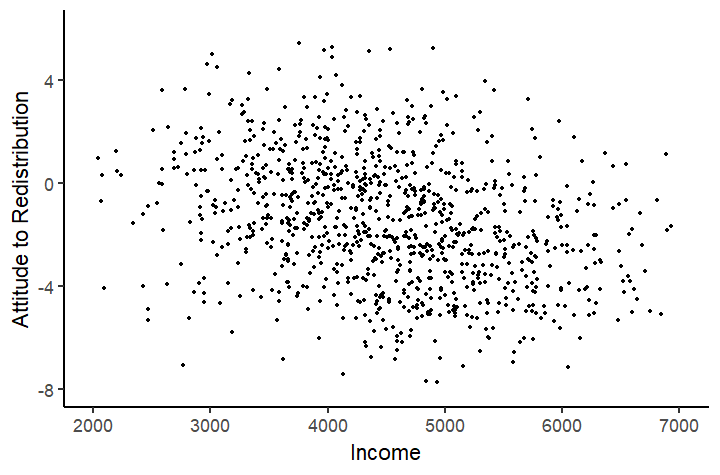
\includegraphics[width=\maxwidth]{figure/confound3b-1} 

\end{knitrout}
\end{frame}

\begin{frame}
\frametitle{Omitted Variable Bias}
\begin{knitrout}
\definecolor{shadecolor}{rgb}{0.969, 0.969, 0.969}\color{fgcolor}
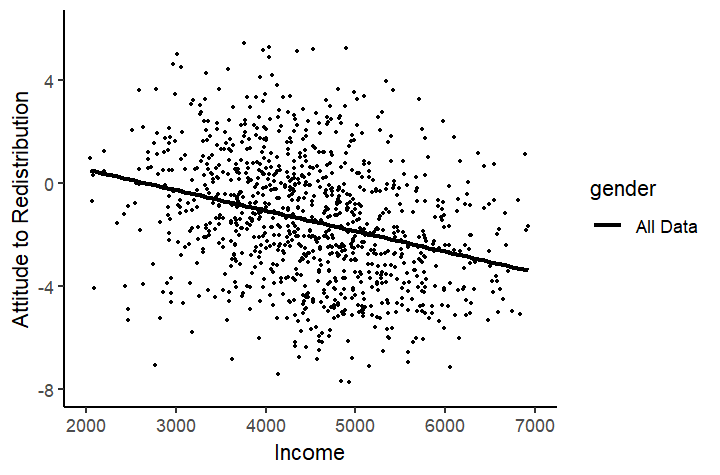
\includegraphics[width=\maxwidth]{figure/confound3c-1} 

\end{knitrout}
\end{frame}

\begin{frame}
\frametitle{Omitted Variable Bias}
\begin{knitrout}
\definecolor{shadecolor}{rgb}{0.969, 0.969, 0.969}\color{fgcolor}
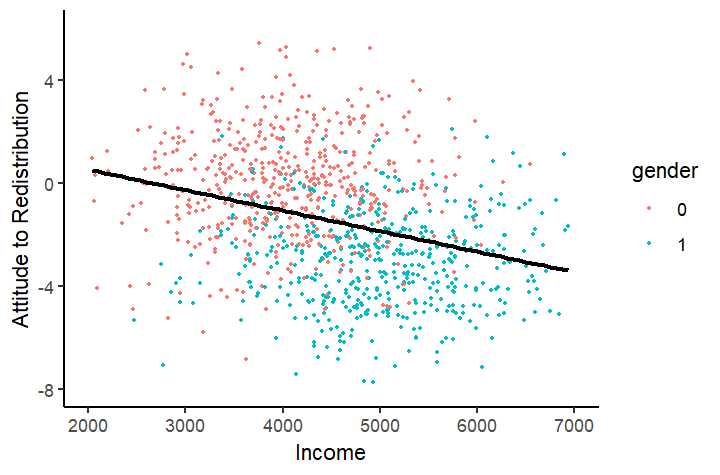
\includegraphics[width=\maxwidth]{figure/confound2-1} 

\end{knitrout}
\end{frame}


\begin{frame}
\frametitle{Omitted Variable Bias}
\begin{knitrout}
\definecolor{shadecolor}{rgb}{0.969, 0.969, 0.969}\color{fgcolor}
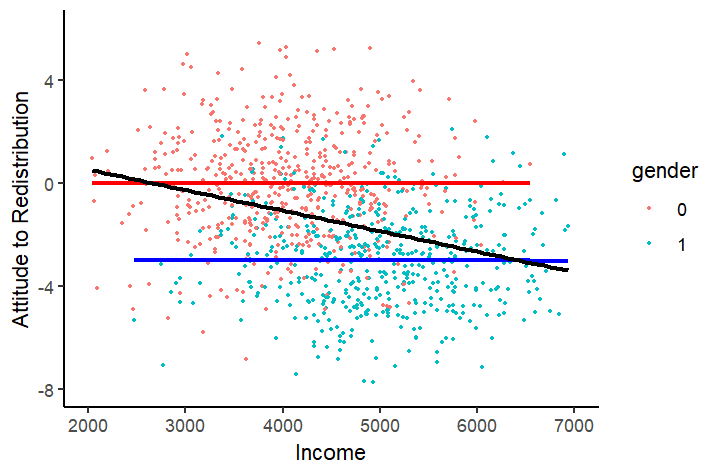
\includegraphics[width=\maxwidth]{figure/confound3-1} 

\end{knitrout}
\end{frame}

% Overlap/Functional form error
% Measurement Error
% Omitted Variable Bias
% Reverse Causation/Endogeneity
% Self-Selection Bias
% Data Selection Bias

% Stress - in prep for week 2 - that regression only buys you (conditional) correlation

%Chenage all examples to age-gender-income

\end{document}


%setwd('C:\\Users\\Jonny\\Google Drive\\Academic\\USP\\Class\\Week 1 - Intro\\Lecture Slides')
%knitr::knit("Slides_Wk1_intro_5.Rnw")
